\documentclass{class-for-drafts}

\usepackage{hyperref}
%% url
\usepackage{url}
%% maths
\usepackage{amsmath}
%%\usepackage{amsfonts}
\usepackage{amssymb}
%% \usepackage{amsthm}
%% algorithms
%\usepackage{algorithm}
\usepackage{algorithmicx}
%\usepackage[noend]{algpseudocode}
\usepackage[ruled, linesnumbered, noend]{algorithm2e}

%% images
\usepackage{graphicx}
%% inparaenum
\usepackage{paralist}

%% tables
\usepackage{booktabs}
\usepackage{multirow}
%% figures
%\usepackage{caption}
\usepackage{subfig}
%\usepackage[font=small, skip=2pt]{caption}
%\usepackage[font=small]{subfig}
\usepackage{tikz}
\usetikzlibrary{arrows.meta,decorations.pathreplacing,decorations.pathmorphing,plotmarks,shapes,matrix}
\tikzset{>={Latex[width=3pt,length=5pt]}}
%% transform eps in pdf crossplateform
\usepackage{epstopdf}
\usepackage{epsfig}
%% hyphenation
\usepackage{hyphenat}
\hyphenation{brow-sers brow-ser}

\newcommand{\TODO}[1]{\textcolor{red}{#1}}
\newcommand{\REF}[0]{\textcolor{purple}{REF}}

\usepackage{xspace}
\newcommand{\SCAMP}[0]{\textsc{Scamp}\xspace}
\newcommand{\CYCLON}[0]{\textsc{Cyclon}\xspace}
\newcommand{\SPRAY}[0]{\textsc{Spray}\xspace}
\newcommand{\LSEQ}[0]{\textsc{LSeq}\xspace}
\newcommand{\CRATE}[0]{\textsc{Crate}\xspace}
\newcommand{\PEERSIM}[0]{\textsc{PeerSim}\xspace}

\usepackage{amsthm} %% proof env
\newtheorem{definition}{Definition}
\newtheorem{theorem}{Theorem}

%%%%%%%%%%%%%%%%%%%%%%%%%%%%%%%%%%%%%%%%%%%%%%%%%%%%%%%%%%%%%%%%%%%%%%%%%%%%%%%
%%%%%%%%%%%%%%%%%%%%%%%%%%%%%%%%%%%%%%%%%%%%%%%%%%%%%%%%%%%%%%%%%%%%%%%%%%%%%%%
%%%%%%%%%%%%%%%%%%%%%%%%%%%%%%%%%%%%%%%%%%%%%%%%%%%%%%%%%%%%%%%%%%%%%%%%%%%%%%%


\begin{document}

%\title{A better causal broadcast}
\title{\TODO{Breaking the Scalability Barrier of} Causal Broadcast\\for Large
  and Dynamic Networks}

\newcommand{\affLSNN}{L2SN, University of Nantes\\
  2 rue de la Houssini{\`e}re\\
  BP 92208, 44322 Nantes Cedex 3, France\\
  \url{first.last@univ-nantes.fr}}

\author{Brice N{\'e}delec, Pascal Molli, and Achour Most{\'e}faoui \aff \affLSNN}

\proceedings{}

%\copyright{}

\maketitle


\begin{abstract}
  Many distributed protocols and applications rely on causal broadcast to ensure
  consistency criteria.
  %% However, tracking causality while scaling remains an open
  %% problem. 
  However, none of causality tracking state-of-the-art approaches scale in large
  and dynamic networks.   
  %% State-of-the-art approaches do not scale in large and
  %% dynamic networks.
  % State-of-the-art approaches overload messages with control information the
  % size of which increases linearly compared to either the number of processes,
  % or the number of broadcast messages.
  % These approaches are impracticable in large scale systems subject to churn.
  We present a uniform reliable causal broadcast protocol that outperforms
  state-of-the-art in size of messages, execution time complexity, and local
  space complexity. Most importantly, it does not overload messages with any
  control information.  We prove that this holds in both static and dynamic
  networks.  Consequently, large and dynamic systems can finally afford causal
  broadcast.
\end{abstract}

%\keywords{Uniform, reliable, causal, broadcast.}

% \begin{IEEEkeywords}
% Uniform, reliable, causal, broadcast.
% \end{IEEEkeywords}

%%% Local Variables:
%%% mode: latex
%%% TeX-master: "../paper"
%%% End:


\section{Introduction}

Broadcast is a communication primitive allowing a process to send a message to
all other processes in the network. We can add order on message delivery. It
alleviates the burden of applications to check message relationships. FIFO
broadcast exists but not so useful. Causal broadcast is very useful; many
applications require causal order. Holy grail is total order broadcast but not
scalable, equivalent to consensus.


%%% Local Variables:
%%% mode: latex
%%% TeX-master: "../paper"
%%% End:


\section{Preliminaries}
\label{sec:preliminaries}

\begin{definition}[Process]
  is said correct if it does not crash.
\end{definition}

\begin{definition}[Broadcast]
  
\end{definition}

\begin{definition}[Uniform reliable broadcast]

\begin{asparadesc}
\item [Validity:] If a correct process broadcasts $m$, then it eventually delivers $m$.
\item [Uniform Agreement:] If a process -- correct or not -- delivers $m$, then
  all correct processes eventually deliver $m$.
\item [Uniform Integrity:] $m$ is delivered by a process at most once, and only
  if it was previously broadcast.
\end{asparadesc}

\end{definition}


\begin{definition}[Causal delivery]
  
\end{definition}

\begin{figure}
  \begin{center}
  
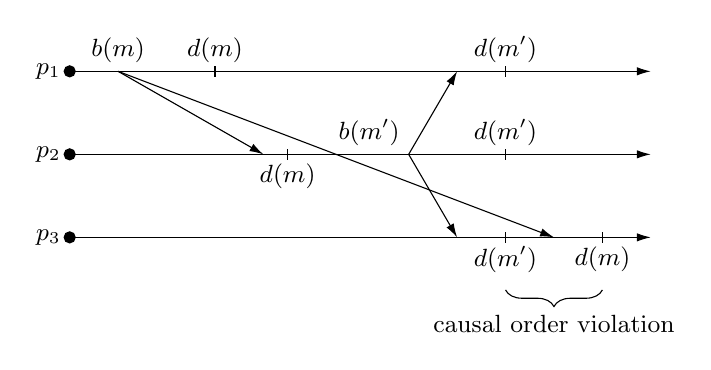
\begin{tikzpicture}[scale=1]
  \small

  \newcommand\X{35pt};
  \newcommand\Y{30pt};
  
  \draw[->](0pt,   0pt)--(6*\X,   0pt);
  \draw[->](0pt, -1*\Y)--(6*\X, -1*\Y);
  \draw[->](0pt, -2*\Y)--(6*\X, -2*\Y);
  
  \draw[fill=black](0pt, 0pt) node[anchor=east]{$p_1$}circle(2pt);
  \draw[fill=black](0pt, -1*\Y) node[anchor=east]{$p_2$}circle(2pt);
  \draw[fill=black](0pt, -2*\Y) node[anchor=east]{$p_3$}circle(2pt);

  \draw[->](0.5 * \X, 0pt)node[anchor=south]{$b(m)$}--(2 * \X,   -1 * \Y);
  \draw[->](0.5 * \X, 0pt)--( 5 * \X,   -2 * \Y);
  \draw(1.5*\X, -2pt)--node[anchor=south]{$d(m)$}(1.5*\X, 2pt);
  \draw(2.25 * \X, -2 -1*\Y )--node[anchor=north]{$d(m)$}(2.25 * \X,    2 -1 * \Y);
  \draw(5.5 * \X, -2 -2*\Y )--node[anchor=north]{$d(m)$}(5.5 * \X,    2 -2 * \Y);

  \draw[->](3.5 * \X, -1*\Y )--(4 * \X,   -2 * \Y);
  \draw[->](3.5 * \X, -1*\Y )node[anchor=south east]{$b(m')$}--(4 * \X,    0 * \Y);
  \draw(4.5 * \X, -2 -0*\Y )--node[anchor=south]{$d(m')$}(4.5 * \X,    2 -0 * \Y);
  \draw(4.5 * \X, -2 -1*\Y )--node[anchor=south]{$d(m')$}(4.5 * \X,    2 -1 * \Y);
  \draw(4.5 * \X, -2 -2*\Y )--node[anchor=north]{$d(m')$}(4.5 * \X,    2 -2 * \Y);
  
  \draw[decorate,decoration={brace,amplitude=6pt,mirror,raise=4pt}]
  (4.5*\X, -2.5*\Y) -- node[anchor=north, yshift=-10pt]{\small causal order violation} (5.5*\X, -2.5*\Y);
\end{tikzpicture}

%%% Local Variables:
%%% mode: latex
%%% TeX-master: "../paper"
%%% End:

  \caption{\label{fig:generalproblem}Broadcast without causal order
    enforcement.}
  \end{center}
\end{figure}

Figure~\ref{fig:generalproblem} depicts an example where causal order is
violated. Process $p_1$ broadcasts and delivers $m$. Process $p_2$ receives and
delivers $m$. Then, it broadcasts and delivers $m'$. Process $p_3$ receives $m'$
before $m$. Without any causal order enforcement, $p_3$ delivers $m'$ before $m$
violating the condition stating that the delivery of $m$ should precede the
delivery $m'$.

Multiple approaches exist to enforce causal order by either piggybacking control
information in each message, or constraining the network topology. In this
paper, we introduce a causal broadcast protocol freed from both these
requirements.


%%% Local Variables:
%%% mode: latex
%%% TeX-master: "../paper"
%%% End:


\section{Causal broadcast}
\label{sec:proposal}

We propose an approach guaranteeing causal order to uniform reliable
broadcasts. It only makes use of FIFO communication channels (e.g. TCP), and
relies on scalable peer-sampling protocols that must not create network
partitions (e.g. \SPRAY~\cite{nedelec2017adaptive}, or
\CYCLON~\cite{voulgaris2005cyclon}).

\TODO{If ok with model section, change this paragraph a bit.}
Section~\ref{subsec:fifobroadcast} starts by showing that FIFO-based broadcast
is sufficient to provide causal delivery of messages. This result holds if the
network is static or links are removed only. It does not hold if links are added
to the network. Section~\ref{subsec:bufferbroadcast} provides a simple algorithm
that solves this issue. It allows processes to use a causal broadcast which
alleviates applications of the burden of tracking causal relationships.

\subsection{2-processes equivalent model}

\begin{figure}
  \begin{center}
    
\begin{tikzpicture}[scale=1]

  \newcommand\X{110pt}
  \newcommand\Y{35pt}
  
  \small
  \draw[fill=white] (0*\X, 0*\Y) node{$p_{from}$} +(-12pt,-12pt) rectangle +(12pt,12pt);
  \draw[fill=white] (1*\X, 0*\Y) node{$p_{to}$} +(-12pt,-12pt) rectangle +(12pt,12pt);
  
  \draw[->](12pt, 12pt) to[out=65, in=180-65] ( -12+ 1*\X, 12pt);
  \draw[->, densely dotted](12pt, 0pt) -- ( -12+ 1*\X, 0pt);
  \draw[->, dashdotted](12pt, -12pt) to[out=-65, in=-180+65] ( -12+ 1*\X, -12pt);

%  \draw[->](12pt, -12pt) to[out=-25, in=-180+25] ( -12+ 1*\X, -12pt);
%  \draw[->, densely dashed](12pt, -12pt) to[out=-35, in=-180+35] ( -12+ 1*\X, -12pt);
%  \draw[->, densely dashdotted](12pt, -12pt) to[out=-65, in=-180+65] ( -12+ 1*\X, -12pt);


\end{tikzpicture}
    \caption{\label{fig:2eqmodel}2-processes equivalent of a broadcast from any
      process to any other.}
    \end{center}
\end{figure}


\subsection{FIFO-based causal broadcast}
\label{subsec:fifobroadcast}

The FIFO-based causal broadcast relies on a peer-sampling protocol. It provides
a set of neighbors to communicate with via FIFO channels. The peer-sampling
protocol must ensure that the network is not partitioned.

\begin{definition}[FIFO communication channel]
  If Process $p$ sends a message $m$ then $m'$ to Process $q$ using a FIFO
  channel, $q$ receives $m$ before $m'$.
\end{definition}

\begin{algorithm}[h]
  
\algblockdefx[initially]{initially}{endInitially}
[0] {\textbf{INITIALLY:}}

\algsetblockdefx[event]{event}{endEvent}
{65535}{}
[0] {\textbf{EVENTS:}}

\algsetblockdefx[dissemination]{dissemination}{endDissemination}
{65535}{}
[0] {\textbf{DISSEMINATION:}}


\newcommand{\comment}[1]{$\rhd$ #1}
\newcommand{\LINEIFTHEN}[2]{%
  \algorithmicif\ {#1}\ \algorithmicthen\ {#2} %
}
\newcommand{\LINEIFTHENELSE}[3]{%
  \algorithmicif\ {#1}\ \algorithmicthen\ {#2} \algorithmicelse\ {#3}%
}

\newcommand{\LINEFOR}[2]{%
  \algorithmicfor\ {#1}\ \algorithmicdo\ {#2} %
}

\begin{algorithmic}[1]

  \initially
  \State $p$ \hfill \comment{This process identity}
  \State $Q$ \hfill \comment{$p$'s neighborhood, FIFO channels}
  \endInitially
  
  \dissemination

  \Function{broadcast} {$m$} \hfill \comment{$b_p(m)$}
  \State \LINEFOR{\textbf{each} $q \in Q$} 
  {$\textsc{sendTo}(q,\, m)$}
  \EndFunction
  
  \Statex

  \Function{forward} {$m$}
  \State \LINEFOR{\textbf{each} $q \in Q$} 
  {$\textsc{sendTo}(q,\, m)$}
  \EndFunction

  \Statex
  
  \Function{receive} {$m$}  
  \If {$\neg \textsc{alreadyReceived}(m)$}
  \State $\textsc{forward}(m)$
  \State $\textsc{deliver}(m)$ \hfill \comment{$d_p(m)$}
  \EndIf

  \EndFunction

\end{algorithmic}


%%% Local Variables:
%%% mode: latex
%%% TeX-master: "../paper"
%%% End:

  \caption{\label{algo:fifobroadcast}FBC-broadcast.}
\end{algorithm}

Algorithm~\ref{algo:fifobroadcast} shows the instructions of the causal
broadcast mechanism built using FIFO channels. Functions $\textsc{broadcast}$
and $\textsc{forward}$ are distinct although holding the same instructions to
highlight that only 1 process broadcasts while all other processes
forward. Function $\textsc{receive}$ makes sure that each process forwards each
message exactly once. Function $\textsc{alreadyReceived}$ checks if a message
has already been received by the process. We voluntarily keep the implementation
out of this paper, for it constitutes an orthogonal problem. It is worth noting
that this feature is achievable without overhead in terms of message size.

\begin{definition}[Static network]
  A network is static if it comprises an unmutable set of edges and an unmutable
  set of processes.
\end{definition}

% \paragraph{Static networks.} A network is a set of processes linked by a set
% of channels. In a static network, processes cannot fail nor leave, and links
% cannot be created nor removed. In this context, FIFO channels are sufficient
% to provide causal ordering of messages.

\begin{theorem}[\label{theo:static}FBC-broadcast in static networks is causal]
  Assuming a static network without partitions, FBC-broadcast is causal.
\end{theorem}

\begin{proof} \TODO{Prove validity, uniform agreement, uniform integrity?} To
  prove causal ordering, we must show that such broadcast provides both FIFO
  ordering and Local ordering of messages. \\
  \textbf{FIFO:} Suppose a process $p$ broadcasts $m$ before $m'$. Consider that
  a correct process $q$ delivers $m'$. We must show that $q$ delivers $m$ before
  $m'$. Process $p$ broadcast message $m$ before broadcasting $m'$ to all its
  neighborhood using FIFO channels. Each neighbor eventually receives and
  delivers $m$ then $m'$. Each neighbor forwards each message exactly once in
  the order they delivered them to all its neighbors using FIFO channels. Since
  we assume a network without clusters, messages reach all processes. Process
  $q$ eventually receives and delivers $m$ first, then it eventually receives
  and delivers $m'$. \\
  \textbf{Local:} Suppose a process $p$ delivers $m$ before broadcasting
  $m'$. Consider a correct process $q$ that delivers $m'$. We must show that $q$
  delivers $m$ before $m'$. Since $p$ delivers $m$ before broadcasting $m'$, it
  forwards $m$ to all its neighbors before broadcasting $m'$ to the same
  neighbors. Similarly to FIFO ordering, due to the use of FIFO channels, the
  forwardings, and the absence of network clusters, Process $q$ already received
  or eventually receives $m$ when it receives $m'$. Thus, it delivers $m$ before
  delivering $m'$. \\
  \textbf{Causal:} From Theorem~\ref{theo:causal}, since FBC-broadcast ensures
  both FIFO ordering and Local ordering, it ensures Causal ordering.
\end{proof}


\begin{figure}
  \begin{center}
    \input{./input/figstatic.tex}
    \caption{\label{fig:static}FIFO channels are sufficient to provide causal
      order in static networks.}
  \end{center}
\end{figure}

\paragraph{\emph{Example.}}Figure~\ref{fig:static} shows FBC-broadcast solves
the causal order violation from Figure~\ref{fig:generalproblem} by using FIFO
channels.  The figure shows a static network comprising 3 processes $p_1$,
$p_2$, and $p_3$ linked to each other. The figure does not show messages sent by
$p_3$ for the sake of clarity.  The processes receive $m$ and $m'$ multiple
times but there exist no link in the paths from $p_2$ to $p_3$ that carries $m'$
without having carried $m$ beforehand. Hence, the delivery of $m$ always
precedes the delivery of $m'$ at any process.

% \paragraph{Dynamic networks.} Removing a channel does not impair causal
% ordering of messages except if it generates network
% partitions. \TODO{Theorem.}

\begin{definition}[Dynamic network]
  A network is dynamic if it comprises a mutable set of edges and a mutable set
  of processes.
\end{definition}

\begin{theorem}[FBC-broadcast in dynamic networks subject to link removal is
  causal]
  As long as the network is not partitioned, FBC-broadcast remains causal when
  the number of links in the network is monotonically decreasing.

%%  \TODO{In fact, it
%%    remains causal even when partitionned. But uniform agreement is violated.}
\end{theorem}

\begin{proof}
  Removing a link does not change the delivery order of causally related
  messages. Proof of Theorem~\ref{theo:static} about causal order holds.
  However, removing a link may create network partitions. In such case, a
  message may not reach all processes. FBC-broadcast still ensures causal order,
  but uniform agreement is violated.
  % Consider Process $p$ belongs to partition $A$, Process $q$ belongs to
  % partition $B$. Messages broadcast by processes of Partition $A$ reach
  % processes of Partition $B$, but not the converse, assuming links are
  % unidirectional. Processes $p$ broadcasts a message $m$ received and delivered
  % by $q$. Then $q$ broadcasts a message $m'$
  % As long as the removal of links do not partition the network, messages reach
  % all processes. The proof is therefore identical to that of
  % Theorem~\ref{theo:static}.
\end{proof}

\begin{theorem}[\label{theo:removals}FBC-broadcast in dynamic network subject to link additions is
  not causal]
  Using FBC-broadcast, adding links to the network may lead to causal order
  violations.
\end{theorem}

\begin{figure}
  \begin{center}
    \input{./input/figproblem.tex}
    \caption{\label{fig:problem}Adding a FIFO channel endangers causal
      ordering.}
  \end{center}
\end{figure}

\begin{figure}
  \begin{center}
    
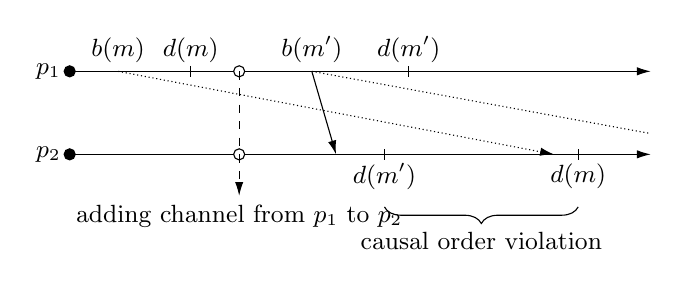
\begin{tikzpicture}[scale=1]
  \small

  \newcommand\X{210/6pt};
  \newcommand\Y{30pt};

  \draw[->](0pt,   0pt)--(6*\X,   0pt);
  \draw[->](0pt, -1*\Y)--(6*\X, -1*\Y);
%%  \draw[->](0pt, -2*\Y)--(6*\X, -2*\Y);
 
  \draw[fill=black](0pt, 0pt) node[anchor=east]{$p_1$}circle(2pt);
  \draw[fill=black](0pt, -1*\Y) node[anchor=east]{$p_2$}circle(2pt);
%  \draw[fill=black](0pt, -2*\Y) node[anchor=east]{$p_3$}circle(2pt);


  \draw[->, densely dotted](0.5*\X, 0pt)node[anchor=south]{$b(m)$}--(5*\X, -1*\Y);
  \draw(1.25*\X, 2pt)--node[anchor=south]{$d(m)$}(1.25*\X, -2pt);
  \draw(3.25*\X, -2-1*\Y )--node[anchor=north]{$d(m')$}(3.25*\X, 2-1*\Y);

%  \draw[->](3*\X, -1*\Y)--(5*\X, -2*\Y);
%%  \draw(5.25*\X, -2-2*\Y )--node[anchor=north]{$d(m)$}(5.25*\X, 2-2*\Y);

  \draw[fill=white](1.75*\X, 0pt) circle(2pt);
  \draw[fill=white](1.75*\X, -1*\Y) circle(2pt);

  \draw[->, dashed](1.75*\X, 0pt) -- (1.75*\X, -1.5*\Y)
  node[anchor=north]{adding channel from $p_1$ to $p_2$};

  \draw[->](2.5*\X, 0pt)node[anchor=south]{$b(m')$} -- (2.75*\X, -1*\Y);
  \draw(3.5*\X, -2pt )--node[anchor=south]{$d(m')$}(3.5*\X, 2pt);
  \draw[densely dotted](2.5*\X, 0pt) -- (6*\X, -0.75*\Y);
%%  \draw(3.25*\X, -2-2*\Y )--node[anchor=north]{$d(m')$}(3.25*\X, 2-2*\Y);
  \draw(5.25*\X, -2-1*\Y )--node[anchor=north]{$d(m)$}(5.25*\X, 2-1*\Y);


  \draw[decorate,decoration={brace,amplitude=6pt,mirror,raise=4pt}] (3.25*\X,
  -1.5*\Y) -- node[anchor=north, yshift=-10pt]{\small causal order violation}
  (5.25*\X, -1.5*\Y);

%%  \draw(5*\X, -1*\Y)--(6*\X, -1.5*\Y);

  
\end{tikzpicture}

    \caption{\label{fig:eq2problem}2-processes equivalent problem of
      Figure~\ref{fig:problem}.}
  \end{center}
\end{figure}

\begin{proof}
  Figure~\ref{fig:problem} illustrates the issue with the establishment of new
  FIFO channels. In this example, a FIFO channel links $p_1$ to $p_2$; another
  links $p_2$ to $p_3$; none links $p_1$ to $p_3$. Other FIFO channels may exist
  but we do not show them for the sake of simplicity. Process $p_1$ broadcasts
  $m$ and delivers it. $p_3$ receives it by the intermediary of $p_2$. In the
  meantime, $p_1$ creates a FIFO channel to $p_3$, then broadcasts $m'$ to $p_2$
  and $p_3$. Since the path through $p_2$ is longer in terms of propagation time
  compared to the direct connections from $p_1$ to $p_3$, Process $p_3$ receives
  and delivers $m'$ before $m$. It violates causal order, for $m'$ precedes $m$.
\end{proof}

Handling dynamic networks is mandatory for causal broadcast
mechanisms. Unfortunately, FBC-broadcast fails when links are added to the
network. Staying with the principle of FIFO-based broadcast, we extend
FBC-broadcast to fully handle dynamic networks. The solution is lightweight and
only uses local knowledge.

\subsection{FIFO-based causal broadcast+}
\label{subsec:bufferbroadcast}

The issue is that new links can act as shortcut for messages. This may create
gaps in causal delivery, i.e., messages that should be delivered are still
missing.  FIFO-based causal broadcast$^+$ aims to ensure that additional links
never create gaps. The idea is to employ already working FIFO channels to know
which messages arrived, at marginal cost. For instance, assuming that we have
$d_p(m) \rightarrow d_p(m')$ and $d_p(m') \rightarrow d_p(m'')$, if Process $p$
knows that Process $q$ received and delivered at least $m$, it can send $m'$
then $m''$ to Process $q$. Any subsequent message from $p$ becomes safe to
travel through the newly added link.

%%Knowing that at least Message $m$ arrived allows the process to send
%%depending messages $m'$, $m''$ 


Solving this issue requires 3 steps. When a process $p$ wants to use a link to a
process $q$ for causal broadcast,
\begin{enumerate}[(i)]
\item it must use the FIFO channels already in use to transmit a message to $q$
  awaiting for its acknowledgment.
\item While awaiting for this acknowledgment, $p$ buffers each message it
  sends.
\item When $p$ receives the acknowledgment from $q$, it uses the FIFO channel
  from $p$ to $q$ to send its buffered messages. Afterwards, the channel is
  ready to be used for causal broadcast.
\end{enumerate}

\begin{algorithm}[h]
  
\SetKwProg{Function}{function}{}{}
\SetKwProg{Upon}{upon}{}{}
\SetKwProg{Initially}{INITIALLY:}{}{}
\SetKwProg{Dissemination}{DISSEMINATION:}{}{}
\SetKwProg{Safety}{SAFETY:}{}{}

\small

\DontPrintSemicolon
\LinesNumbered

\Initially {} {
  $Q$ \tcp*{$p$'s neighborhood, FIFO channels}
  $B \leftarrow \varnothing$ \tcp*{Buffers of messages}
}

\BlankLine

\Safety {} {
  \Upon{\textsc{open}($q$)} {
    \If{$|Q|>1$} {
      $Q \leftarrow Q \setminus q$ \;
      $B[q] \leftarrow \varnothing$ \;
      $\textsc{sendLocked}(p,\, q)$ \;
    }
  }
  
  \BlankLine
  
  \Upon{\textsc{receiveLocked}($from, \, to$) \tcp*[f]{$to=p$}} {
    $\textsc{sendAck}(from,\, to)$ \;
  }
  
  \BlankLine

  \Upon{\textsc{receiveAck}($from,\, to$) \tcp*[f]{$from=p$}} {
    \If {$to \in B$} {
      \lForEach {$m \in B[to]$} {$\textsc{sendTo}(to,\, m)$}
      $B \leftarrow B \setminus to$ \;
      $Q \leftarrow Q \cup to$ \;
    }
  }

  \BlankLine

  \Upon{\textsc{close}($q$)} {
    $B \leftarrow B \setminus q$ \;
  }

}

\BlankLine

\Dissemination {} {

  \Function{\textsc{FBC-broadcast}$^+$($m$) \tcp*[f]{$b_p(m)$}} {    
    \lForEach {$q \in B$} {$B[q] \leftarrow B[q] \cup m$ \tcp*[f]{Buffers}}
    $\textsc{R-broadcast}(m)$ \;
  }
  
  \BlankLine
  
  \Upon{\textsc{R-deliver}($m$)} {
    \lForEach {$q \in B$} {$B[q] \leftarrow B[q] \cup m$ \tcp*[f]{Buffers}}
    $\textsc{FBC-deliver}(m)$ \tcp*{$d_p(m)$}
  }

}


%%% Local Variables:
%%% mode: latex
%%% TeX-master: "../paper"
%%% End:

  \caption{\label{algo:bufferbroadcast}FBC-broadcast$^+$.}
\end{algorithm}


Algorithm~\ref{algo:bufferbroadcast} shows the instructions of our improved
FIFO-based causal broadcast. Similarly to Algorithm~\ref{algo:fifobroadcast},
each process has a set of neighbors to communicate with via FIFO
channels. Messages transitively reach all processes using forwarding. Processes
deliver and forward each message exactly once.  

Compared to Algorithm~\ref{algo:fifobroadcast}, it adds a structure associating
each opening channel with a buffer of messages. When Process $p$ gets notified
that another FIFO channel to Process $q$ is available, it associates this
channel with an empty buffer of messages. It also sends a \emph{locked} message
to $q$. We leave aside the implementation of this send function (e.g. broadcast
or routing), but it must use the FIFO channels already in use.  Process $p$ does
not use the new links until Process $q$ confirmed the receipt of the locked
message. Acknowledgments do not have to travel through FIFO channels.  Once it
receives the acknowledgment, $p$ empties the buffer of messages to $q$ and start
using the channel normally.

\begin{theorem}[FBC-broadcast$^+$ is causal]
  As long as the network is not partitioned, FBC-broadcast$^+$ is causal in both
  static and dynamic networks.
\end{theorem}

\begin{proof}
  For static and dynamic networks with link removals, the proof is identical to
  that of Theorems~\ref{theo:static} and~\ref{theo:removals}, for the buffers do
  not activate in such instances. For dynamic networks with link additions, we
  must show that FBC-broadcast$^+$ ensures both
  FIFO order and Local order. \\
  \textbf{FIFO:} \TODO{meow} \\
  \textbf{Local:} \TODO{miaw} \\
  \textbf{Causal:} From Theorem~\ref{theo:causal}, since FBC-broadcast$^+$
  ensures both FIFO ordering and Local ordering, it ensures Causal ordering.
\end{proof}

\begin{figure}
  \begin{center}
    \input{./input/figsolved.tex}
    \caption{\label{fig:solved}FBC-broadcast$^+$ in dynamic networks. $m'$
      cannot precede $m$.}
  \end{center}
\end{figure}

\begin{figure}
  \begin{center}
    
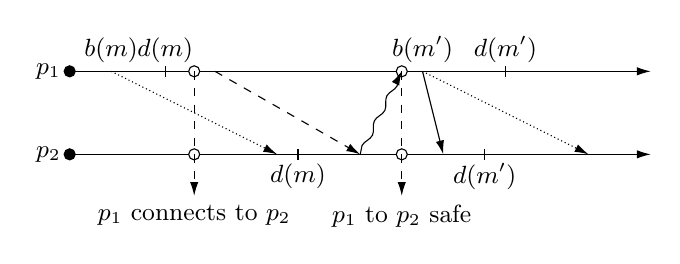
\begin{tikzpicture}[scale=1]
  \small

  \newcommand\X{210/7pt};
  \newcommand\Y{30pt};
  
  \draw[->](0pt,   0pt)--(7*\X,   0pt);
  \draw[->](0pt, -1*\Y)--(7*\X, -1*\Y);
%%  \draw[->](0pt, -2*\Y)--(7*\X, -2*\Y);
  
  \draw[fill=black](0pt, 0pt) node[anchor=east]{$p_1$}circle(2pt);
  \draw[fill=black](0pt, -1*\Y) node[anchor=east]{$p_2$}circle(2pt);
%%  \draw[fill=black](0pt, -2*\Y) node[anchor=east]{$p_3$}circle(2pt);
  
  
  \draw[->, densely dotted](0.5*\X, 0pt)node[anchor=south]{$b(m)$}--(2.5*\X, -1*\Y);
  \draw(1.15*\X, 2pt)--node[anchor=south]{$d(m)$}(1.15*\X, -2pt);
  \draw[->, dashed](1.75*\X, 0*\Y) -- (3.5*\X, -1*\Y);
%  \draw(2.25*\X, 2 -1*\Y)--node[anchor=south]{$d(m)$}(2.25*\X, -2 - 1*\Y);
  
%  \draw[->](2*\X, -1*\Y)--(2.5*\X, -2*\Y); %% p2 -> m -> p3
  \draw(2.75*\X, 2 -1*\Y)--node[anchor=north]{$d(m)$}(2.75*\X, -2 - 1*\Y);
  
%%  \draw[->, dashed](3*\X, -1*\Y)--(3.5*\X, -2*\Y); %% p2 -> l -> p3
  
  \draw[fill=white](4*\X, 0pt) circle(2pt);
  \draw[fill=white](4*\X, -1*\Y) circle(2pt);
  \draw[->, dashed](4*\X, 0pt) -- (4*\X, -1.5*\Y)
  node[anchor=north]{$p_1$ to $p_2$ safe};
  
  \draw[->, decorate, decoration={snake, amplitude=0.3mm}](3.5*\X, -1*\Y)--(4*\X, 0); %% p3 -> a -> p1
  
  %% \draw(3.25*\X, -2-1*\Y )--node[anchor=south]{$d(m)$}(3.25*\X, 2-1*\Y);
  
  %% \draw[->](3*\X, -1*\Y)--(5*\X, -2*\Y);
  %% \draw(5.25*\X, -2-2*\Y )--node[anchor=north]{$d(m)$}(5.25*\X, 2-2*\Y);

  \draw[fill=white](1.5*\X, 0pt) circle(2pt);
  \draw[fill=white](1.5*\X, -1*\Y) circle(2pt);
  \draw[->, dashed](1.5*\X, 0pt) -- (1.5*\X, -1.5*\Y)
  node[anchor=north]{$p_1$ connects to $p_2$};


  \draw[->](4.25*\X, 0pt)node[anchor=south]{$b(m')$} -- (4.5*\X, -1*\Y);
  \draw(5.25*\X, 2pt)--node[anchor=south]{$d(m')$}(5.25*\X, -2pt);
  \draw(5*\X, 2 - 1*\Y)--node[anchor=north]{$d(m')$}(5*\X, -2 - 1 *\Y);
  \draw[->, densely dotted](4.25*\X, 0pt) -- (6.25*\X, -1*\Y); %% p1 -> m' -> p2
%  \draw(6.25*\X, 2 - 1*\Y)--node[anchor=south]{$d(m')$}(6.25*\X, -2 - 1 *\Y);
%%  \draw[->](5.75*\X, -1*\Y) -- (6.25*\X, -2*\Y); %% p2 -> m' -> p


  % \draw[->](2.5*\X, 0pt)node[anchor=south]{$b(m')$} -- (2.75*\X, -2*\Y);
  % \draw(3.5*\X, -2pt )--node[anchor=south]{$d(m')$}(3.5*\X, 2pt);
  % \draw[->](2.5*\X, 0pt) -- (5*\X, -1*\Y);
  % \draw(3.25*\X, -2-2*\Y )--node[anchor=north]{$d(m')$}(3.25*\X, 2-2*\Y);
  % \draw(5.25*\X, -2-1*\Y )--node[anchor=south]{$d(m')$}(5.25*\X, 2-1*\Y);


  % \draw[decorate,decoration={brace,amplitude=6pt,mirror,raise=4pt}] (3.25*\X,
  % -2.5*\Y) -- node[anchor=north, yshift=-10pt]{\small causal order violation}
  % (5.25*\X, -2.5*\Y);

  %% \draw(5*\X, -1*\Y)--(6*\X, -1.5*\Y);

  
\end{tikzpicture}

    \caption{\label{fig:eq2solved}2-processes equivalent of Figure~\ref{fig:solved}.}
  \end{center}
\end{figure}

\paragraph{\emph{Example.}} Figure~\ref{fig:solved} shows how our algorithm
solves causal order violations. Similarly to Figure~\ref{fig:problem}, a FIFO
channel links $p_1$ to $p_2$; another link $p_2$ to $p_3$; none links $p_1$ to
$p_3$. Process $p_1$ broadcasts $m$. Then $p_1$ wishes to create a link to
$p_3$. It sends a message to $p_3$ using its FIFO channels. Thus, $m$ precedes
this message at $p_3$. When $p_3$ acknowledges this message to $p_1$ using any
communication way, the later knows that it $p_3$ received and delivered at least
$m$. Hence, all subsequent broadcast from $p_1$ can use the new communication
channel safely. When $p_1$ broadcasts $m'$, there exist no path where $m'$
arrives before $m$.

\begin{figure}
  \begin{center}
    
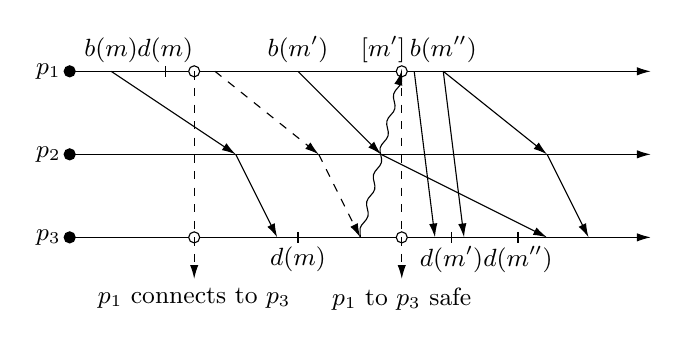
\begin{tikzpicture}[scale=1]
  \small

  \newcommand\X{210/7pt};
  \newcommand\Y{30pt};

  \draw[->](0pt,   0pt)--(7*\X,   0pt);
  \draw[->](0pt, -1*\Y)--(7*\X, -1*\Y);
  \draw[->](0pt, -2*\Y)--(7*\X, -2*\Y);
 
  \draw[fill=black](0pt, 0pt) node[anchor=east]{$p_1$}circle(2pt);
  \draw[fill=black](0pt, -1*\Y) node[anchor=east]{$p_2$}circle(2pt);
  \draw[fill=black](0pt, -2*\Y) node[anchor=east]{$p_3$}circle(2pt);

  
  \draw[->](0.5*\X, 0pt)node[anchor=south]{$b(m)$}--(2*\X, -1*\Y);
  \draw(1.15*\X, 2pt)--node[anchor=south]{$d(m)$}(1.15*\X, -2pt);
  \draw[->, dashed](1.75*\X, 0*\Y) -- (3*\X, -1*\Y);

  \draw[->](2*\X, -1*\Y)--(2.5*\X, -2*\Y); %% p2 -> m -> p3
  \draw[->, dashed](3*\X, -1*\Y)--(3.5*\X, -2*\Y); %% p2 -> l -> p3

  \draw[fill=white](4*\X, 0pt) circle(2pt);
  \draw[fill=white](4*\X, -2*\Y) circle(2pt);
  \draw[->, dashed](4*\X, 0pt) -- (4*\X, -2.5*\Y)
  node[anchor=north]{$p_1$ to $p_3$ safe};

  \draw[->, decorate, decoration={snake, amplitude=0.3mm}](3.5*\X, -2*\Y)--(4*\X, 0); %% p3 -> a -> p1
  
  \draw(2.75*\X, 2 -2*\Y)--node[anchor=north]{$d(m)$}(2.75*\X, -2 - 2*\Y);
  
  \draw[fill=white](1.5*\X, 0pt) circle(2pt);
  \draw[fill=white](1.5*\X, -2*\Y) circle(2pt);
  \draw[->, dashed](1.5*\X, 0pt) -- (1.5*\X, -2.5*\Y)
  node[anchor=north]{$p_1$ connects to $p_3$};

  %% p1 -> m' -> p1
  \draw[->](2.75*\X, 0pt)node[anchor=south]{$b(m')$} -- (3.75*\X, -1*\Y); 
  \draw[->](3.75*\X, -1*\Y) -- (5.75*\X, -2*\Y); %% p2 -> m' -> p3

  %% p2 -> [m] -> p3
  \draw[->](4.15*\X, 0*\Y)node[anchor=south east]{[$m'$]} -- (4.4*\X, -2*\Y);
  \draw(4.6*\X, 2 -2*\Y)--node[anchor=north]{$d(m')$}(4.6*\X, -2 - 2*\Y);

  %% p2 -> m'' -> p3
  \draw[->](4.5*\X, 0*\Y) node[anchor=south]{$b(m'')$}-- (4.75*\X, -2*\Y);
  \draw[->](4.5*\X, 0*\Y) -- (5.75*\X, -1*\Y); %% p1 -> m'' -> p2
  \draw[->](5.75*\X, -1*\Y) -- (6.25*\X, -2*\Y); %% p2 -> m'' -> p3
  \draw(5.4*\X, 2 -2*\Y)--node[anchor=north]{$d(m'')$}(5.4*\X, -2 - 2*\Y);

  % \draw[->](2.5*\X, 0pt)node[anchor=south]{$b(m')$} -- (2.75*\X, -2*\Y);
  % \draw(3.5*\X, -2pt )--node[anchor=south]{$d(m')$}(3.5*\X, 2pt);
  % \draw[->](2.5*\X, 0pt) -- (5*\X, -1*\Y);
  % \draw(3.25*\X, -2-2*\Y )--node[anchor=north]{$d(m')$}(3.25*\X, 2-2*\Y);
  % \draw(5.25*\X, -2-1*\Y )--node[anchor=south]{$d(m')$}(5.25*\X, 2-1*\Y);


  % \draw[decorate,decoration={brace,amplitude=6pt,mirror,raise=4pt}] (3.25*\X,
  % -2.5*\Y) -- node[anchor=north, yshift=-10pt]{\small causal order violation}
  % (5.25*\X, -2.5*\Y);

  %% \draw(5*\X, -1*\Y)--(6*\X, -1.5*\Y);

  
\end{tikzpicture}

    \caption{\label{fig:buffer}Role of the buffer in FBC-broadcast$^+$ during
      link addition. $m''$ cannot precede $m'$. \TODO{Not done.}}
  \end{center}
\end{figure}

\begin{figure}
  \begin{center}
    \input{./input/figeq2buffer.tex}
    \caption{\label{fig:eq2buffer}2-processes equivalent of
      Figure~\ref{fig:buffer}.}
  \end{center}
\end{figure}

\paragraph{\emph{Example.}} The previous example does not depict the buffer
usage. The buffer becomes useful when a process broadcast a message between the
opening of a channel and the receipt of the corresponding
acknowledgment. Figure~\ref{fig:buffer} shows an example where a process uses a
buffer to ensure causal delivery of messages. 


\TODO{not done.}


\paragraph{Complexity.} For each process, the \emph{local space complexity} is
that of the buffers which is unbounded by default and depends of the
peer-sampling protocol, network conditions, and broadcast frequencies. It is
worth noting that the size of buffer can be bounded, i.e., above a threshold,
either the buffer is cleared and another locked message is sent waiting for an
acknowledgment, or the communication channel is removed altogether.

There is no overhead in the \emph{size of messages}. 

Since each process broadcasts or forwards a message exactly once to all its
neigbhors, the \emph{number of messages} generated by each process for each
broadcast is $|Q|-|B|$. 

The \emph{traffic} generated by each process for each broadcast is
$(|Q|-|B|)*|m|$. 

The \emph{number of hops} for a message to reach all peers depends of the
peer-sampling protocol. Using a random peer-sampling protocol, we can reach a
logarithmic bound.


%%% Local Variables:
%%% mode: latex
%%% TeX-master: "../paper"
%%% End:


\section{Related work}
\label{sec:relatedwork}

\TODO{Table comparing the improvement. Local overhead. Number of
  messages. Message overhead.}

\paragraph{Vector clock-based approaches.}
\paragraph{Topological contraint-based approaches.}

\paragraph{Inter-group
  broadcast~\cite{johnson1998scalable,johnson1999intergroup}.} Explain the link
between this approach and our approach (every peer is an inter-group router).


%%% Local Variables:
%%% mode: latex
%%% TeX-master: "../paper"
%%% End:


\section{Conclusion}
\label{sec:conclusion}

% In this paper, we described a uniform reliable causal broadcast that removes the
% need for messages to carry any control information. To handle dynamic networks,
% our approach only requires the help of buffers the size of which can be bounded
% easily. \TODO{Meow meow meow.}


In this paper, we described a uniform reliable causal broadcast protocol that
breaks scalability barriers. Its space complexity remains small and can be
bounded easily. It does not overload messages with any control information. This
result means that large and dynamic systems can finally afford causal broadcast.

% This makes our causal broadcast suitable for large scale networks subject to
% churn.

% Applications and protocols such as distributed data stores, distributed
% collaborative editors that need to track causal relationships between operations
% can now rely on our causal broadcast.


As future work, we plan to investigate on reducing the space complexity of
reliable broadcast. Section~\ref{subsec:complexity} reviews structures with
linearly increasing space consumption. We can reduce this complexity in static
networks. We can prune the structure from already received messages, for we know
that the number of duplicates is equal to the number of incoming links. As for
FIFO-based broadcast, this does not hold in dynamic networks. We would like to
investigate on a way to prune the structure in such settings. This would make
causal broadcast fully scalable as well on generated traffic as on space
consumption.

% As future work, we plan to investigate on the problem of duplicated message
% detection. Although it only impacts local space complexity, this is the last and
% only remaining linear complexity.

% A possible way of improvement lies in the fact that, in static network, each
% process knows how many duplicates of each message it will receive. We could use
% this information to prune the structure of already received
% messages. Unfortunately, it does not hold in dynamic networks.


%% It is awesome.



%%% Local Variables:
%%% mode: latex
%%% TeX-master: "../paper"
%%% End:


% \input{input/acknowledgment.tex}

%%\bibliographystyle{abbrv}
\bibliography{bibliographie}
  
\end{document}

